\section{Method}\label{sec:method}

\subsection{System and preprocessing}

Figure~\ref{fig:pipeline} shows the system. Olivetti images enter a raw-pixel branch (flattened 4096-d; PCA to 2-D for presentation) and a frozen-embedding branch (preprocess, embed, the same PCA settings for presentation); both feed a shared evaluation module that computes every metric in native dimensionality. The live path reuses the embedding branch with MTCNN on CPU and embedding on Apple MPS.

Both paths must produce the same input domain, because the network's standardisation is part of the model (Figure~\ref{fig:preprocess}). For Olivetti, each $64\times64$ greyscale image in $[0,1]$ is replicated to three identical channels, bilinearly resized to $160\times160$ with antialiasing, multiplied by 255, and standardised by
\begin{equation}
x\mapsto \frac{x-127.5}{128}.
\label{eq:standardisation}
\end{equation}
The resize invents no detail, and the recipe reproduces the reference implementation exactly on the 400-image batch. For webcam frames, MTCNN detects a face box with a three-stage cascade, crops and resizes a square to $160\times160$; the library then converts the crop to a $[0,1]$ tensor and applies its fixed standardisation $x\mapsto(x\cdot255-127.5)/128$, which is equivalent to $(x-127.5)/128$ on the original $0$--$255$ intensities. The library crops the O-Net box and does not warp on the five landmarks, so alignment is detector-box alignment; MTCNN runs on CPU because its operations are unsupported on MPS.

\begin{figure}[t]
\centering
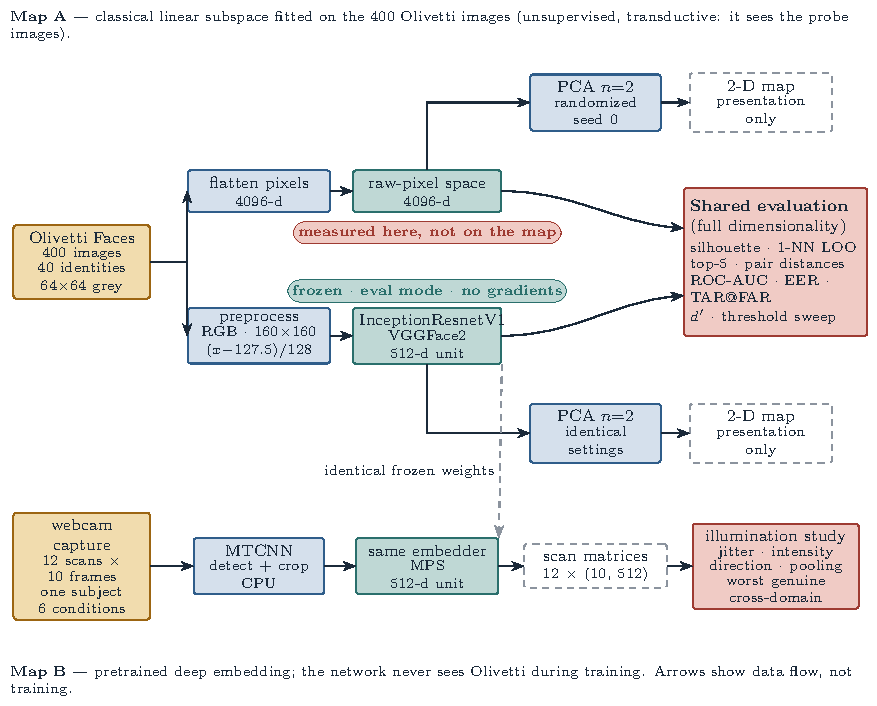
\includegraphics[width=0.78\textwidth]{fig_pipeline.pdf}
\caption{End-to-end system. Raw-pixel branch (Map A), frozen-embedding branch (Map B), and the live webcam path. The 2-D PCA maps are for inspection only; all metrics are computed on the full 4096-d and 512-d vectors before projection. The plot PCA is fitted transductively on all 400 images; full-dimensional scores use the unprojected vectors. Map B's frozen network was pretrained on a separate corpus.}
\label{fig:pipeline}
\end{figure}

\begin{figure}[t]
\centering
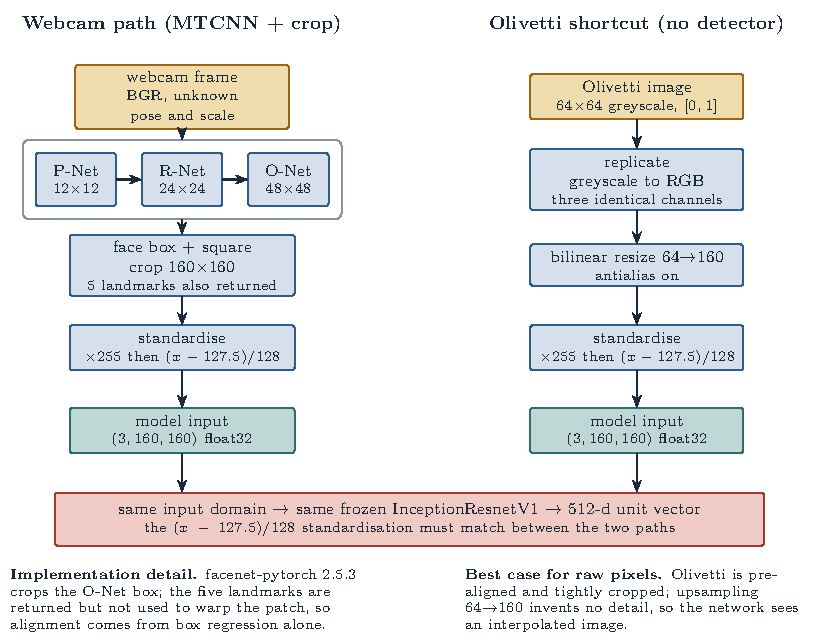
\includegraphics[width=0.78\textwidth]{fig_preprocess.pdf}
\caption{The two preprocessing paths. Webcam (left): MTCNN detects and crops, then the network's fixed standardisation is applied. Olivetti (right): no detector; greyscale is replicated to RGB, resized 64$\to$160 with antialiasing, and standardised identically. The $(x-127.5)/128$ step is part of the model definition.}
\label{fig:preprocess}
\end{figure}

\subsection{Frozen embedder and PCA maps}

Figure~\ref{fig:model} shows Inception-ResNet-v1 \citep{szegedy2017} with tensor shapes measured by forward hooks on the actual VGGFace2 checkpoint \citep{cao2018,facenetpytorch}. A seven-operation stem is followed by five Inception-ResNet-A blocks (Block35, scale 0.17) at $256\times17\times17$, reduction A (\texttt{mixed\_6a}) to $896\times8\times8$, ten Inception-ResNet-B blocks (Block17, scale 0.10), reduction B (\texttt{mixed\_7a}) to $1792\times3\times3$, five Inception-ResNet-C blocks (Block8, scale 0.20) plus a final C block without ReLU, global average pooling to 1792, a bias-free linear layer and batch normalisation to 512, and L2 normalisation. The model is in evaluation mode with gradients disabled, so embedding is deterministic up to hardware arithmetic, and embeddings are cached.

Both 2-D maps use PCA with two components, randomised SVD, seed 0, and sklearn's default centring \citep{pedregosa2011}; the same settings, colours, and style are used for both. We deliberately do not apply \texttt{StandardScaler}: all 4096 pixel columns share one unit, so per-column scaling would inflate near-constant background pixels and change the variance ordering for reasons unrelated to identity; classic Eigenfaces centres but does not standardise. The same implementation produces the explained-variance analysis and the eigenface images; the 2-D coordinates are never a metric input. A rank control projects the raw pixels onto their full rank of 399 components (400 centred samples span at most rank 399), which preserves Euclidean distances exactly (maximum absolute difference $3.5\times10^{-12}$) and reproduces Map A's metrics to numerical precision. This shows that Map A's nominal 4096-dimensionality is not itself the source of its metrics, but it does not match the two spaces (399 versus 512) or control their intrinsic geometry; this check cannot determine whether dimensionality contributes to the raw-versus-embedding gap, which is measured rather than mechanistically attributed.

\begin{figure}[t]
\centering
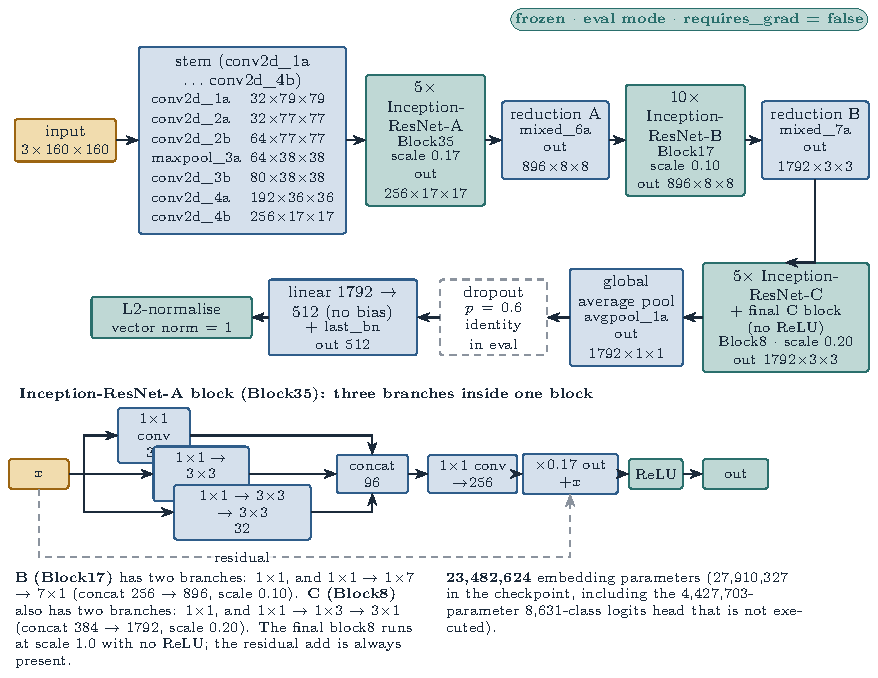
\includegraphics[width=0.78\textwidth]{fig_model.pdf}
\caption{Inception-ResNet-v1 embedding network. Shapes are measured from \texttt{results/model\_arch.json} (forward hooks on the VGGFace2 checkpoint, batch dimension dropped) and follow \texttt{facenet-pytorch} 2.5.3 naming. The model is frozen: evaluation mode, no gradients, 23,482,624 embedding parameters. The inset shows the Inception-ResNet-A block; B and C have two branches each, with kernel shapes and scales given in the note.}
\label{fig:model}
\end{figure}

\subsection{Metrics and protocols}\label{sec:metrics}

Distances are Euclidean; for unit vectors, cosine similarity is $1-d^2/2$. The silhouette score is
\begin{equation}
s(i)=\frac{b(i)-a(i)}{\max\{a(i),b(i)\}},\qquad S=\frac{1}{N}\sum_{i=1}^{N}s(i),
\label{eq:silhouette}
\end{equation}
with $a(i)$ the mean distance to the same identity and $b(i)$ the mean distance to the nearest other identity, on full-dimensional vectors. \emph{1-NN leave-one-out} finds each image's nearest neighbour among the other 399, excluding self; top-5 asks whether the true identity is among the five nearest. \emph{Pair-level} analysis scores all $\binom{400}{2}=79{,}800$ unordered pairs: 1,800 genuine (40 identities $\times\binom{10}{2}$) and 78,000 impostor. FAR and FRR at threshold $\tau$ are
\begin{equation}
\mathrm{FAR}(\tau)=\frac{\#\{d_{\mathrm{imp}}\le\tau\}}{N_{\mathrm{imp}}},\qquad
\mathrm{FRR}(\tau)=\frac{\#\{d_{\mathrm{gen}}>\tau\}}{N_{\mathrm{gen}}},
\label{eq:farfrr}
\end{equation}
from which we report ROC-AUC, EER and its threshold, TAR at FAR $=10^{-3}$ and $10^{-2}$, and $d'$ from Equation~\ref{eq:dprime}. \emph{2-D fidelity} is the Spearman rank correlation between 2-D and full-dimensional pairwise distances over 20,000 seeded pairs. The \emph{confusion analysis} compares 1-NN predictions across maps; with zero Map B errors the ``both wrong'' fraction has an empty denominator and is \texttt{null}, not zero.

The map comparison uses every image once. Verification uses the known-population (closed-set) protocol in Figure~\ref{fig:protocol}: for each of the 40 identities, five images enrol and the other five are held-out probes. Every score is the \emph{minimum} Euclidean distance from a query image to the five enrolment images of the claimed identity, and the decision is accept if the score is at most $\tau$. Genuine trials use each identity's five held-out probes as queries; impostor trials use each of the 390 images of the other 39 identities as queries against the same enrolment set. The primary result averages five random 5/5 splits (seeds 0--4), giving 200 genuine and 15,600 impostor trials per split, identical for both representations. All identities are known and enrolled, so there are no unknown-identity probes and the reported FAR is cross-identity error within a closed population. We report per-split EER, TAR at FAR $=10^{-3}$ and $10^{-2}$, AUC, and FAR at matched 1\% FRR, plus a fixed first-half/second-half split (session-bias check) and a mean-template score rule (sensitivity check). These numbers are descriptive, in-sample, known-population cross-identity estimates: every impostor is one of the same 40 enrolled identities, thresholds are chosen and evaluated on the same scores, and EER is interpolated between observed thresholds rather than a realizable operating point. They are not open-set or deployment estimates. An additive identity-disjoint check, with thresholds chosen on calibration identities and evaluated on disjoint and unknown-to-gallery identities, is reported in Section~\ref{sec:results}.

\begin{figure}[t]
\centering
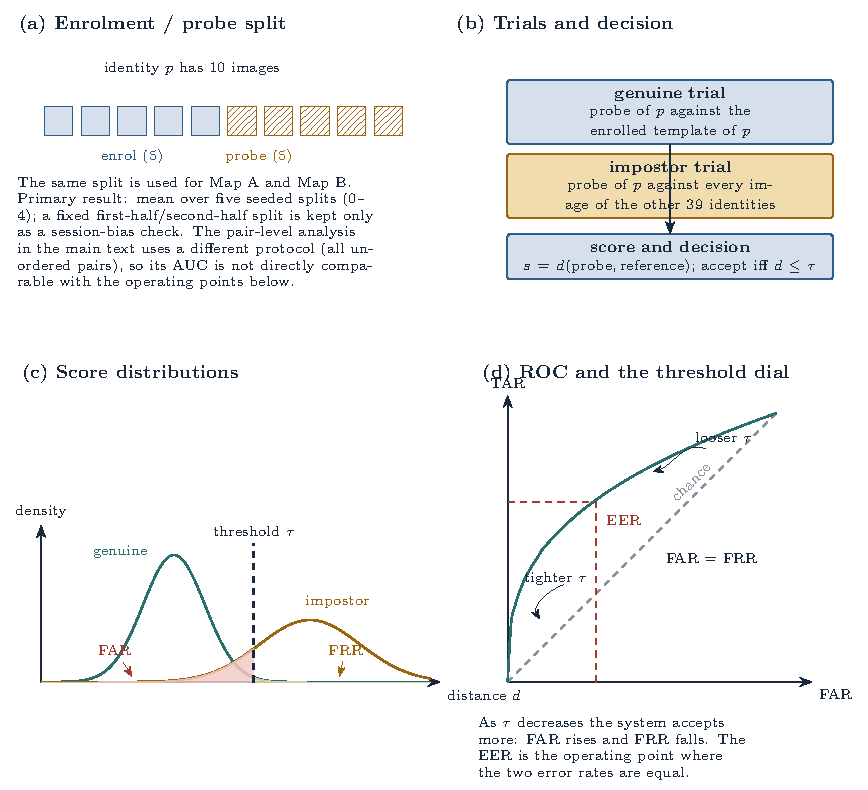
\includegraphics[width=0.78\textwidth]{fig_protocol.pdf}
\caption{Evaluation protocol. (a) Per identity, five images enrol and five probe; the split is identical for both maps. (b) Genuine and impostor trial definitions. (c) Score distributions with threshold $\tau$; FAR is impostor mass at or below $\tau$, FRR is genuine mass above it. (d) ROC curve and the security--convenience dial: raising the distance threshold $\tau$ admits more genuine probes and more impostors, while lowering $\tau$ is tighter. Curves in (c) and (d) are schematics, not measured data.}
\label{fig:protocol}
\end{figure}

\subsection{Live protocol and measurement rule}

The twelve scans are analysed at frame and scan level (Figure~\ref{fig:lighting-setup}). \emph{Within-scan jitter} is the mean of all 45 frame-pair distances inside a scan: the frame-to-frame noise floor. \emph{Same-condition between-scan} distance compares the repeat scans of each condition. The named \emph{intensity comparison} contrasts room-front and flash-front frames; the named \emph{direction comparison} averages the six flash-direction pairs, and the descriptive ratio divides it by within-scan jitter. Different scans and uncontrolled pose/exposure prevent causal interpretation. \emph{Pooling} compares frame-level distances with distances between re-normalised scan means. The \emph{worst genuine} pair is the largest same-person frame-pair distance, with its cosine equivalent and the same quantity after scan averaging. The \emph{cross-domain} check measures distances from the 400 Olivetti embeddings to the live scans; it is domain-confounded and reported only as a descriptive distance, not as a calibrated impostor distribution and neither as an upper nor a lower bound on webcam-domain stranger distance.

\emph{Measure in full dimensionality, plot in 2-D}: no metric is computed on PCA coordinates, and the rank correlation quantifies what the plot loses. \emph{One pipeline}: load, embed, project, plot, score, with only the representation swapped. All experiments use seed 0 unless a protocol averages seeds 0--4; reported measurements are manually transcribed from machine-written JSON and require consistency review after regeneration. Hardware and versions are in Section~\ref{sec:repro}.

\begin{figure}[t]
\centering
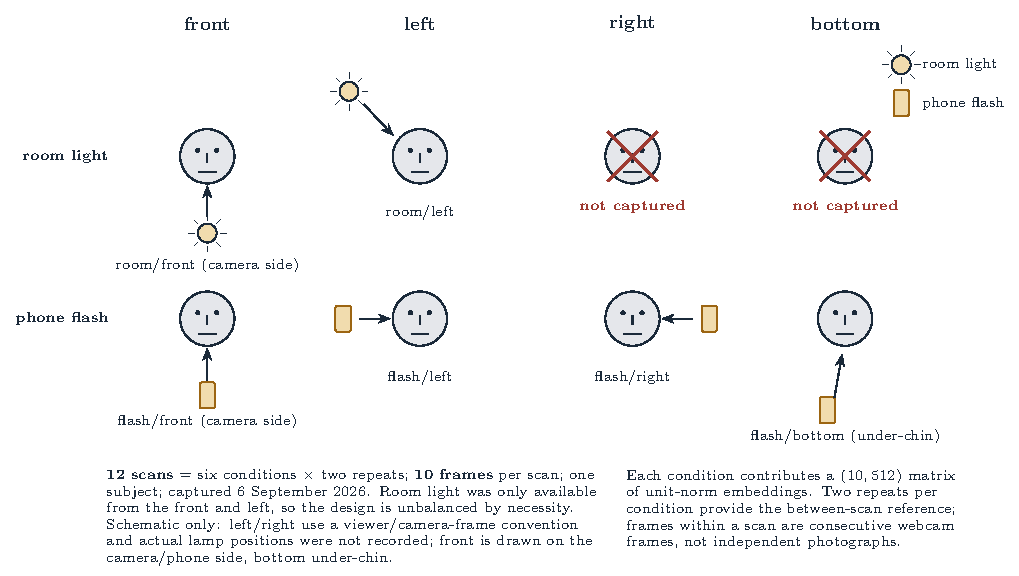
\includegraphics[width=0.92\textwidth]{fig_lighting_setup.pdf}
\caption{Webcam capture conditions. Room light and phone flash were used from up to four directions; room light was only available from front and left, so the design is unbalanced by necessity. Each captured condition has two repeat scans of ten consecutive frames; early frames are affected by webcam warm-up. The left/right placements are a schematic convention (viewer/camera frame) and do not reconstruct the actual lamp positions from the capture; this records the design, not empirically verified geometry.}
\label{fig:lighting-setup}
\end{figure}
